
\begin{figure}[tb]
  \centering
  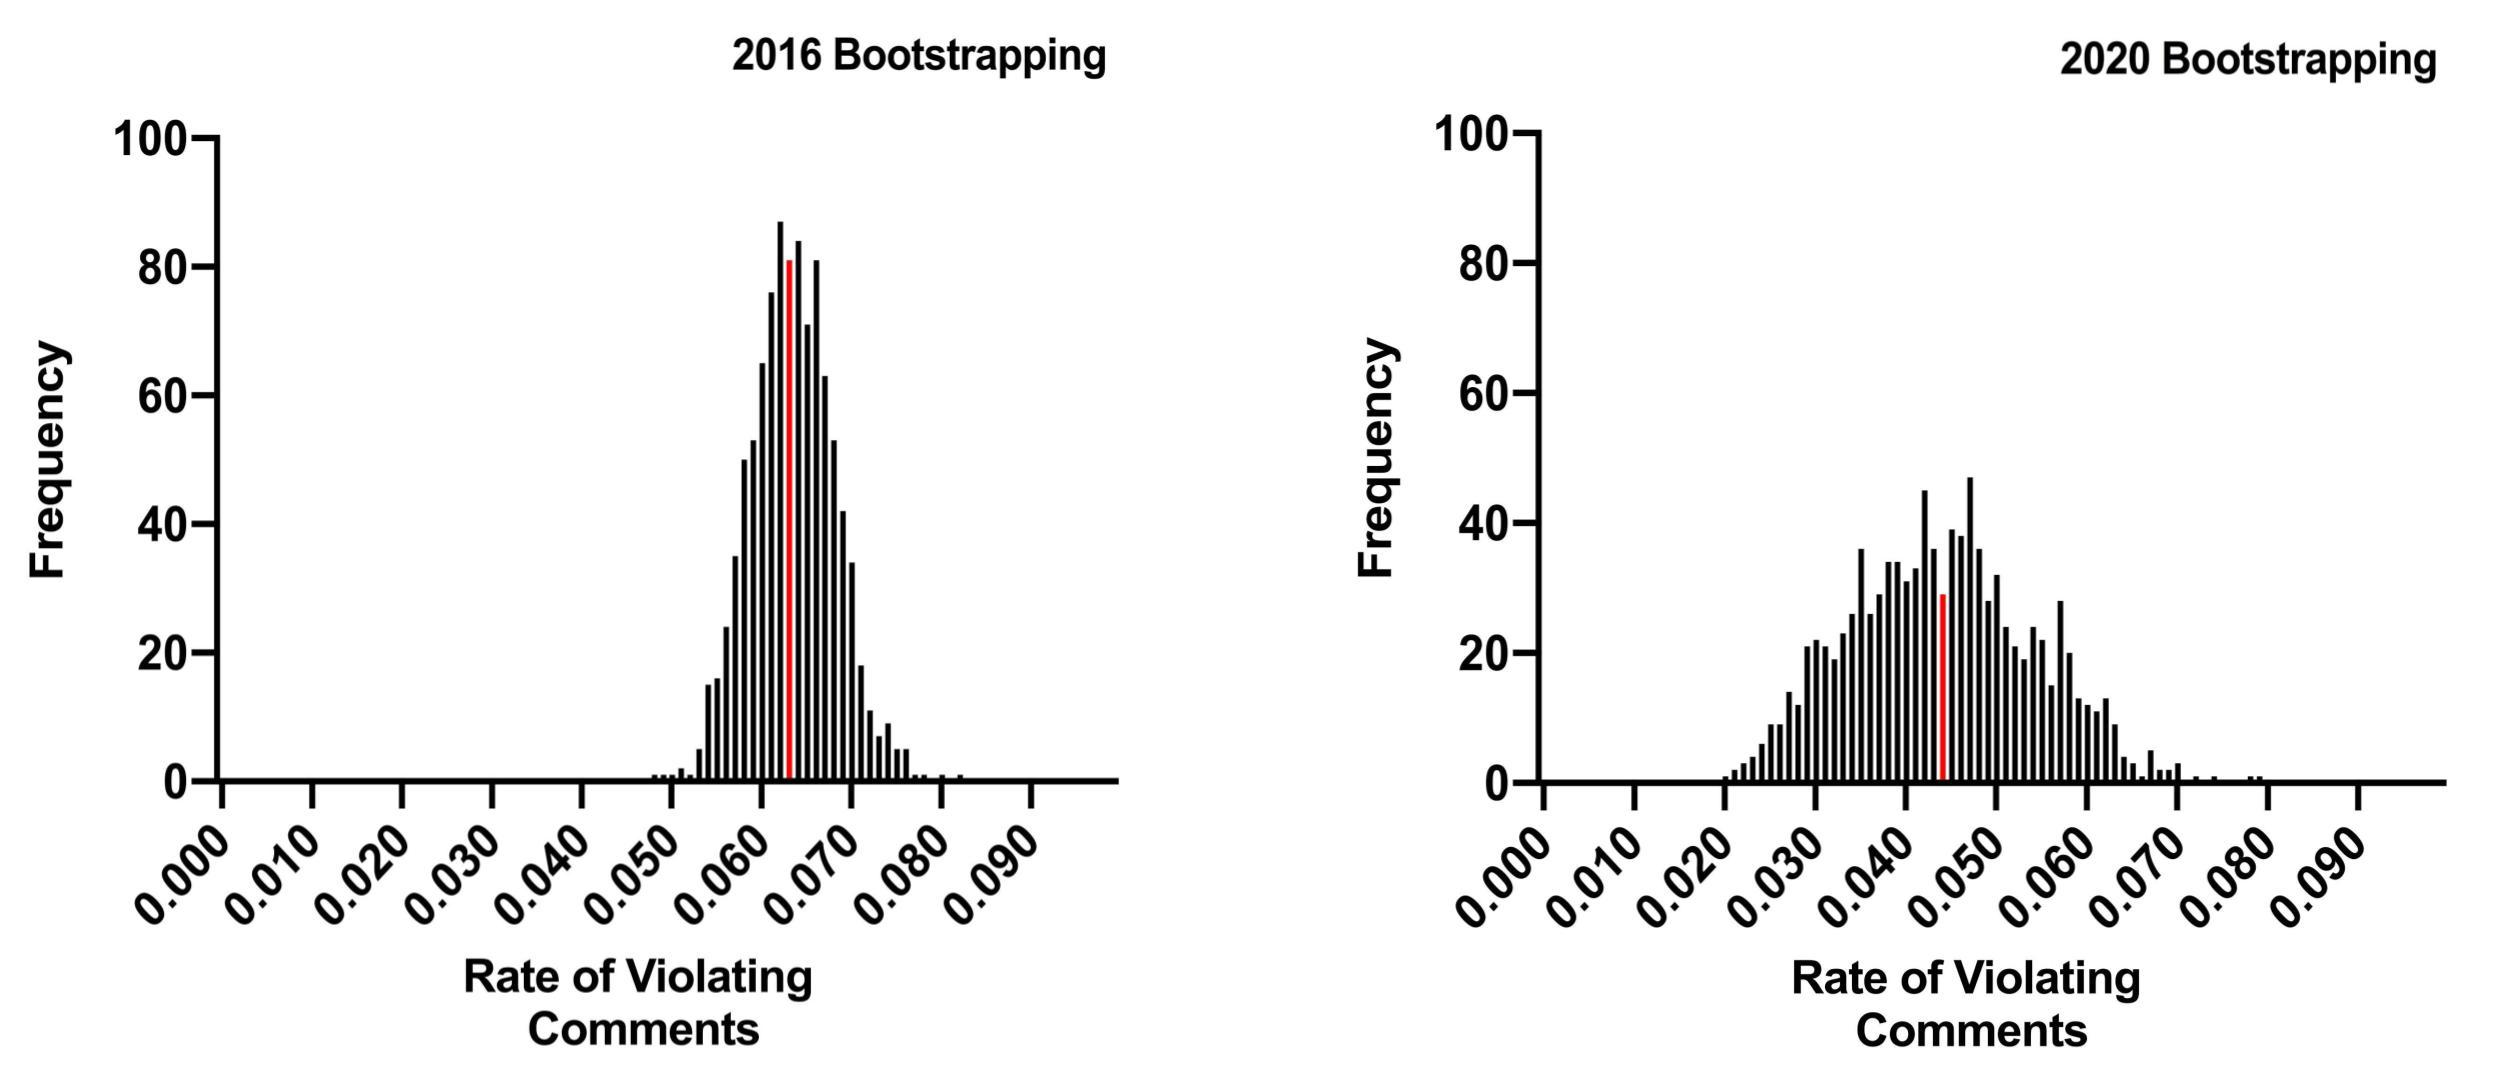
\includegraphics[width=0.95\textwidth]{content_minor_revision__Apr2022/images/bootstrap_rate.jpg}
  \caption{The results of our bootstrap sampling. The figures show the overall rates of violating comments that are left unmoderated for all 1,000 simulations of Reddit for $T_{2016}$ and $T_{2020}$. The 50th percentile rates for the 1,000 bootstrap samples are colored red for the two periods.}
  \label{fig:bootstraprate}
  \Description{Annotation Interface}
\end{figure}
 
\begin{figure}[tb]
  \centering
  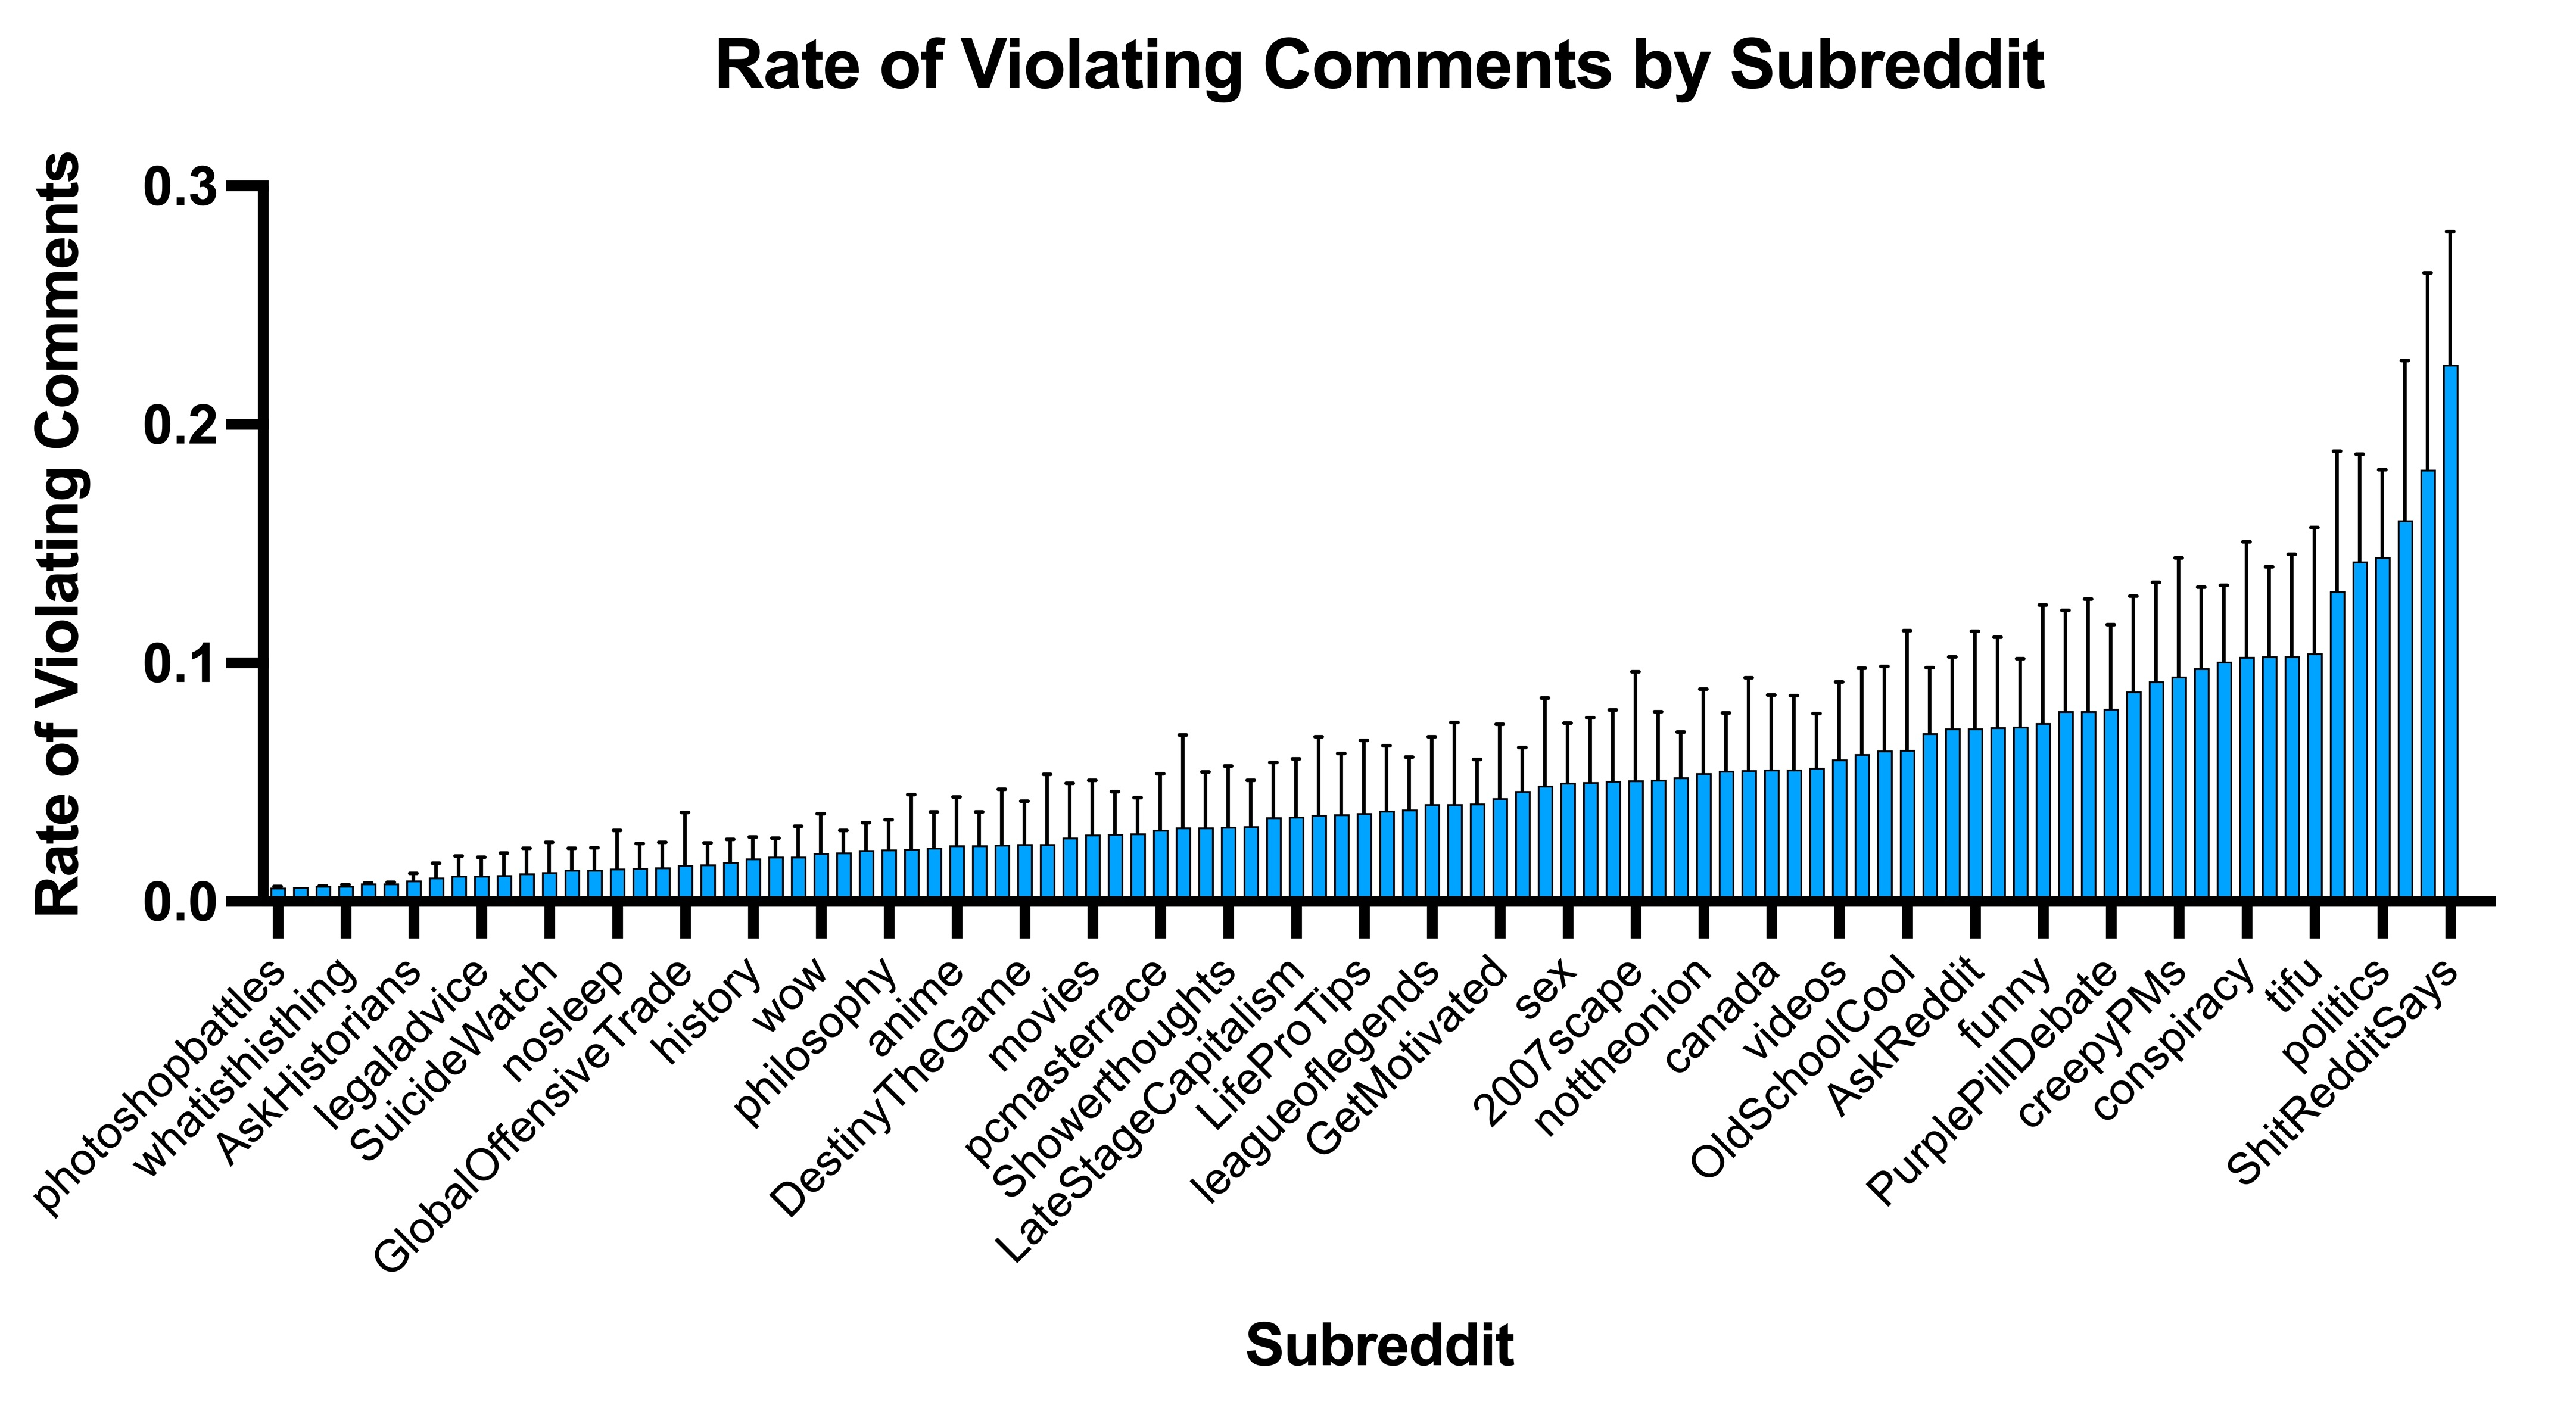
\includegraphics[width=0.95\textwidth]{content_minor_revision__Apr2022/images/all_rate_of_violating.jpg}
  \caption{Rate of \rnr{macro norm} violating comments by subreddit in $T_{2016}$. The lighter lines indicate 95\% confidence intervals. Subreddits vary in levels of violating content; some subreddits like r/depression (1.10\%) and r/Android (1.42\%) contain almost no  \rnr{violating} comments online, whereas some like r/creepyPMs (9.42\%) and r/EnoughTrumpSpam (14.27\%) contains much higher rates of \rnr{violating} comments.}
  \Description{Rate of macro norm violating comments by subreddits}
\end{figure}


\section{RESULTS}

In this section, we present the results of our analyses. We start by reporting on the prevalence of violating comments across our study subreddits and then describe their characteristics in terms of their content, rate of engagement, and language usage.

\subsection{Prevalence of Violating Comments}

\subsubsection{Macro norm violating comments are common}
Figure~\ref{fig:bootstraprate} reports the rate of macronorm violating comments across our 1,000 bootstrap iterations. In $T_{2016}$, 6.25\% (95\% CI [5.36\%, 7.13\%]) of all unmoderated comments are violations. In $T_{2020}$, 4.28\% (95\% CI [2.50\%, 6.26\%]) of all unmoderated comments are violations. \rnr{There are fewer macro norm violating comments over time: a permutation test confirms that the rate of macro norm violating comments is lower in $T_{2020}$ than $T_{2016}$ ($p<.001$).} 

\subsubsection{\rnr{Ablation analysis of the bootstrap confidence intervals}} 
\rnr{In order to (1) confirm that our bootstrapping procedure widens its confidence intervals as fewer human annotations are available, as it should, and (2) confirm that our current number of annotations is sufficient for our estimation goal, we tested the width of the bootstrap's confidence intervals as we ablated to half the number of human annotations per subreddit. On our full dataset for $T_{2016}$ with 32 human annotations per subreddit, the 95\% confidence interval's width is 1.77\%. When we ablate and halve the number of labels from 32 to 16 per subreddit, the confidence interval's width becomes $T_{2016}$ becomes  2.58\% ([4.60, 7.18], median 5.90\%), a 95\% CI width that is .8\% larger. For our smaller $T_{2020}$ dataset with 8 annotations per subreddit, the 95\% CI width is 3.76\% ([2.50, 6.26]). Here, when we ablate and halve the number of labels from 8 to 4 per subreddit, the 95\% CI width widens to 5.43\% ([1.96, 7.39], median 4.27\%), or 1.67\% wider than the original estimate.}


% \usepackage{booktabs}




\begin{table}[tb]
\centering
\captionof{table}{The results of Poisson regression that predicts the rate of problematic comments in a subreddit. We find that the number of comments in a subreddit, as well as a few of the topic categories are strong predictors of the rate of problematic comments a subreddit may have. The topic "general content", which was included in the model, is not shown as it was used as the baseline dummy variable for the categorical variable.}
\begin{tabular}{lllll} 
\toprule
                               & \textbf{Coefficient} & \textbf{SE} & \textbf{z-score} & \textbf{p-value}  \\ 
\toprule
Intercept                      & -5.919               & 1.249       & -4.740           & < 0.001 (***)      \\
log(mod to comment ratio)      & -0.728               & 0.244       & -2.986           & 0.003 (**)        \\
Topic: Hobbies and Occupations & -2.048               & 0.280       & -7.304           & < 0.001 (***)      \\
Topic: NSFW                    & 1.958                & 0.253       & 7.742            & < 0.001 (***)      \\
Topic: Discussion              & -1.021               & 0.421       & -2.423           & 0.015 (*)         \\
Topic: Politics                & 0.628                & 0.260       & 2.414            & 0.016 (*)         \\
Topic: Humor                   & 0.408                & 0.251       & 1.621            & 0.105             \\
Topic: Lifestyle               & 0.0879               & 0.321       & 0.271            & 0.787             \\
Topic: Educational             & -1.191               & 0.647       & -1.840           & 0.078             \\
Topic: Entertainment           & -0.165               & 0.285       & -0.579           & 0.563             \\
Topic: Technology              & -0.387               & 0.325       & -1.191           & 0.233             \\
Topic: Other                   & 0.692                & 0.324       & 2.135            & 0.033             \\
\bottomrule
\end{tabular}
\end{table}



\rnr{Two observations fall out of this ablation analysis. First, we observe that the width of the confidence interval widens as we have fewer annotated comments per subreddit: from 1.77\% with 32 annotations to 2.58\% with 16 annotations in 2016, and from 3.76\% with 8 annotations to 5.43\% with 4 annotations in 2020. This confirms that bootstrapping is not producing overconfident confidence intervals: the confidence intervals widen as we have fewer and fewer labels. Second, we observe that, for 2016 in particular, 32 labels is far more than necessary for the confidence interval to be tight: the interval does not begin to dissolve until having only four labels per subreddit, and providing more than 32 labels per subreddit will not substantially reduce the width of the confidence interval further. The reason for this stability is that, while the estimate for any particular subreddit may be more uncertain, aggregating over nearly 100 subreddits substantially reduces the overall uncertainty.}



\subsubsection{\rnr{Topic and moderator ratio predict the rate of macronorm violations}}
In this subsection, we focus our efforts on the $T_{2016}$ sample. The rate of \rnr{macro norm} violating comments for individual subreddits averages 4.9\% (std=4.0\%), but there is a large spread across different subreddits (Figure 5). For example, subreddits such as r/AskHistorians (0.90\%; 95\% CI [0.73\%, 1.12\%]) and r/science (1.10\%; 95\% CI [0.70\%, 1.61\%]) had lower rates of macro norm violating comments than ones such as r/atheism (10.06\%; 95\% CI [6.99\%, 13.27\%]) and r/politics (14.46\%; 95\% CI [10.79\%, 18.12\%]). Our Poisson regression model, summarized in Table 3, suggests that these differences are associated with the subreddit's topic and its moderator to comment ratio. More specifically, subreddits on NSFW (p<0.001) or political (p=0.016) topics have higher a rate of violating comments, and those hosting hobbies and occupation topics (p=0.001), or discussion topics (p=0.018) are associated with fewer violating comments. Additionally, higher moderator-to-comment ratios are associated with fewer violating comments (p=0.003). 

Although NSFW and political topics featured a higher rate of macro norm violating comments, this did not mean that subreddits covering topics other than these two necessarily had a small number of macro norm violating comments. When excluding 17 subreddits whose topics were categorized as either NSFW and political, we find that the remaining subreddits still had violating comments at the rate of 5.26\% (95\% CI [4.27\%, 6.39\%]). 



\begin{figure}[tb]
  \centering
  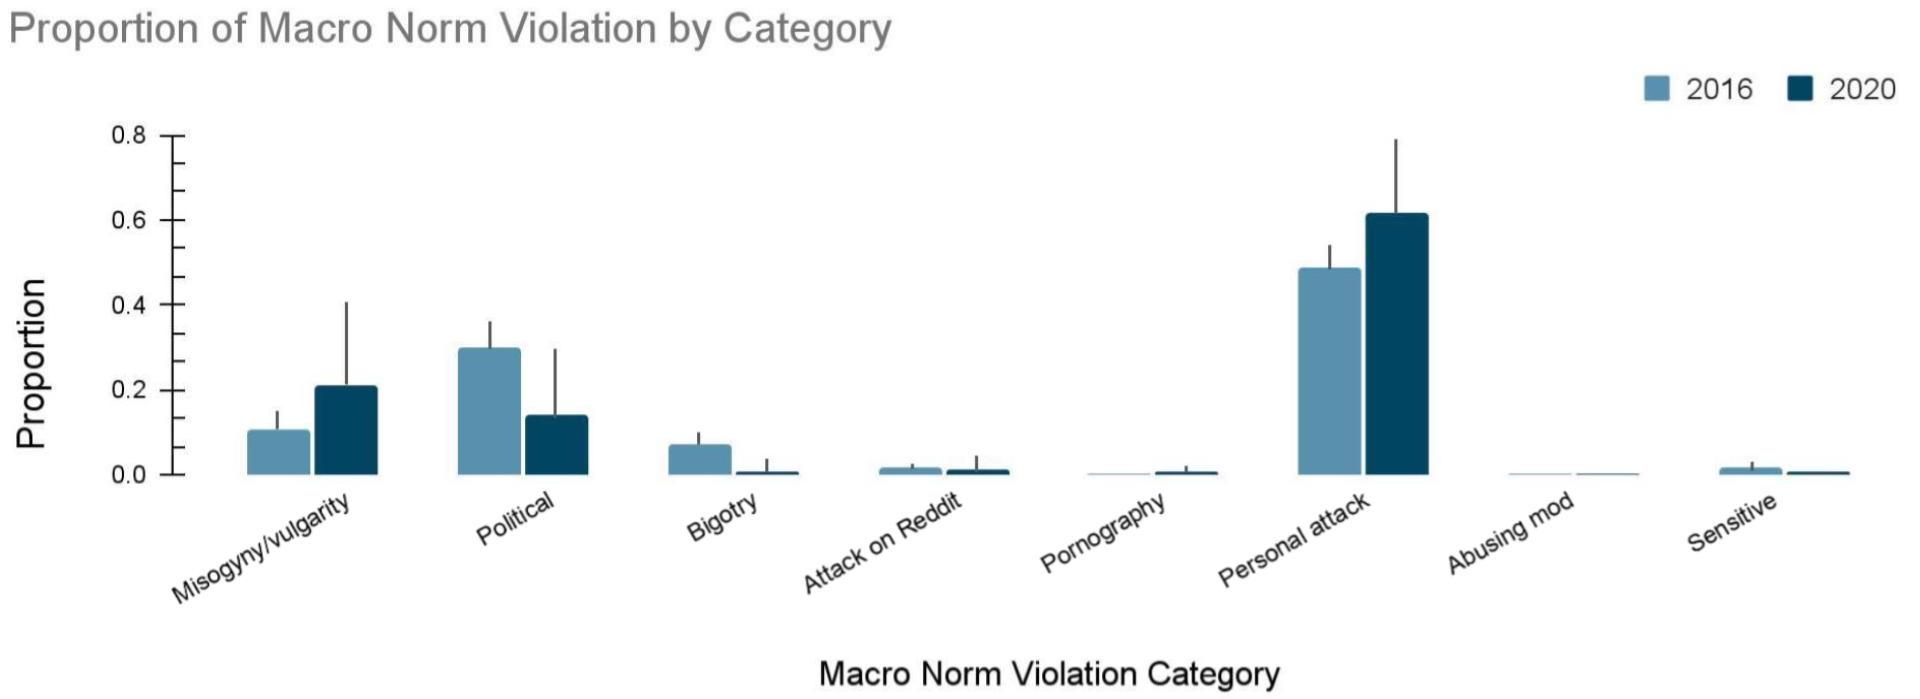
\includegraphics[width=1\textwidth]{content_minor_revision__Apr2022/images/macro_norm_violation_fixed_2.jpg}
  \caption{The proportion of macro norm violation by the eight categories among the unmoderated problematic comments according to our annotators. In $T_{2016}$ as well as $T_{2020}$, personal attacks were the most common macro norm violations. Politically inflammatory comments, on the other hand, have become less prevalent.}
  \Description{Proportion of Macro Norm Violation by Categories}
\end{figure}
% THIS HAS TO BE WITH 6.2.1


\subsection{Characteristics of Violating Comments}
In this subsection, we delve deeper into the violating comments to explicate the categories of violation, engagement rate, and language usage. 



\subsubsection{Personal attacks are the most prevalent category of violation.} 
The eight macronorms are not equally prevalent (Figure 6). In $T_{2016}$, personal attacks (48.58\%; 95\% CI [40.66\%, 56.66\%]) and politically inflammatory comments (30.16\%; 95\% CI [22.80\%, 37.54\%]) are particularly prevalent macronorm violations. On the other hand, categories such as posting pornographic links (<1\%) or abusing moderators (<1\%) were less common. Similarly, in $T_{2020}$, personal attacks (61.94\%; 95\% CI [45.06\%, 80.40\%]) remain the most prevalent, misogyny/vulgarity violations have become more prevalent (20.90\%; 95\% CI [1.33\%, 40.67\%]), and politically inflammatory comments have become less common (14.19\%; 95\% CI [4.49\%, 30.37\%]). 



\subsubsection{Macronorms are moderated at different rates} Moderation removed 4.86\% of macronorm violating comments in 2016–2017, and 10.54\% in 2020. Not all types of macro norm violations were moderated at the same rate, however.
In $T_{2016}$, comments that include links to pornography were moderated at the highest rate (34.53\%), followed by those that abuse or criticize moderators (26.17\%) and those that accuse another of being sensitive (12.87\%). On the other hand, politically inflammatory comments (4.30\%) and misogyny/vulgarity (4.13\%) were less likely to be moderated. Some trends still held in $T_{2020}$, where comments that include pornography were moderated at the highest rate (45.04\%). Nearly all categories were more heavily moderated in 2020 than in 2016.
We summarize the results in Figure 7. 


\subsubsection{Violating comments get fewer upvotes}
We find that in $T_{2016}$, \rnr{macro norm} violating comments garnered an average score of 7.32 (std=21.97), which is significantly lower than the global average of 10.27 (std=95.95) in our dataset according to Welch's t-test (t(469647) = -3.29, p = .001). However, there was no significant difference in the number of top-level replies; the violating comments got 2.00 top-level replies (std=9.25), vs. the global average of 1.92 (std=7.32): t(469647) = 0.21, p=0.83. These result replicate in the $T_{2020}$ sample; the comments that were annotated as violating got an average of 6.07 upvotes (std=13.09), which is significantly lower than the global average of 12.17 (std=119.94) that our sample of 188,000 comments got (t(415515) = -4.30, p < .001). Similarly, there was no significant difference in the number of top-level replies; the violating comments got 1.77 top-level replies (std=2.81) where  1.77 (std=6.82) was the global average (t(415515) = -0.003, p=0.99).


\begin{figure}[tb]
  \centering
  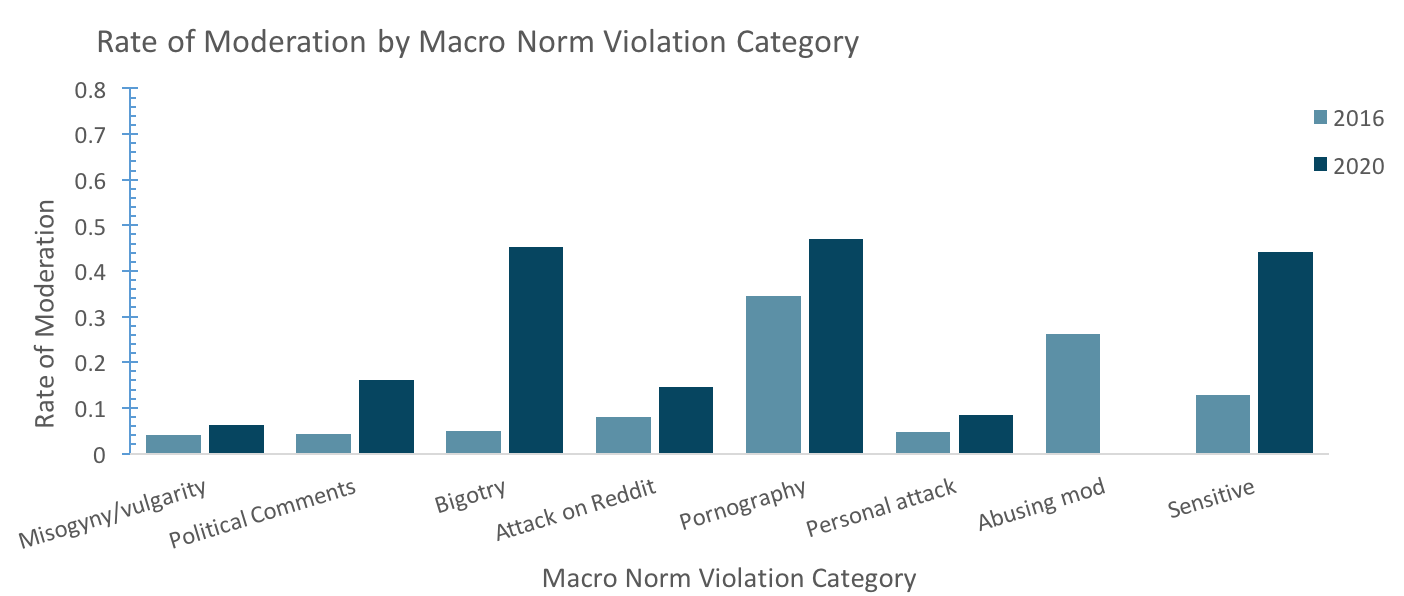
\includegraphics[width=1\textwidth]{content_minor_revision__Apr2022/images/ef_MODERATION.png}
  \caption{The rate of moderation by the eight macro norm violation categories acquired through stratified sampling. In $T_{2016}$, comments that contain links to pornography and comments that abuse or criticize moderators were moderated at the highest rate. In $T_{2020}$, comments with links to pornography is still among the most commonly moderated categories of norm violation. In addition, the overall rate of moderation has increased.  }
  \Description{Rate of moderation by macro norm violation categories}
\end{figure}
% THIS HAS TO BE WITH 6.2.2. AND COME AFTER PROPORTION... 




\subsubsection{More readable and emotional comments are more likely to remain unmoderated} We find that in $T_{2016}$, the readability scores of unmoderated macro norm violating comments averages 62.38 (std=122.51) while the scores of moderated comments averages 33.59 (std=1849.25). Additionally, using Welch's t-test, we confirm that the difference in readability between these two groups of comments is significant (t(2007616)=5.62, p<0.001), indicating that the unmoderated macro norm violating comments are easier to read than the moderated comments. This is replicated in $T_{2020}$, in which the readability scores of the unmoderated macro norm violating comments averages 76.95 (std=31.94) while the scores of moderated comments averages 64.35 (std=293.49). Additionally, this difference between the two groups remains significant (t(160481)=3.59, p<0.001). 

Similarly, we find that in $T_{2016}$, the average emotionality scores of unmoderated macro norm violating comments averages 5.14 (std=1.30) while those of moderated comments averages 0.74 (std=0.51). Once again, the difference in terms of the emotionality score between these two groups of comments is significant according to Welch's t-test (t(378432)=59.89, p<0.001), indicating that the unmoderated macro norm violating comments are more emotional than the moderated comments. This is replicated in $T_{2020}$ in which the average emotionality scores of unmoderated macro norm violating comments averages 4.75 (std=1.40) while those of moderated comments averages 0.80 (std=0.49) with the difference between the two groups being significant (t(74126)=40.90, p<0.001). 


